\documentclass{article}
\usepackage[margin=1in]{geometry}
\usepackage{amsmath}
\usepackage{graphicx}
\usepackage{siunitx}
\usepackage{listings}
\usepackage{xcolor}
\usepackage{hyperref}
\definecolor{mygreen}{rgb}{0,0.6,0}
\definecolor{mygray}{rgb}{0.5,0.5,0.5}
\definecolor{mymauve}{rgb}{0.58,0,0.82}

\lstset{ %
  backgroundcolor=\color{white},   % choose the background color; you must add \usepackage{color} or \usepackage{xcolor}
  basicstyle=\scriptsize\ttfamily,    % the size of the fonts that are used for the code
  breakatwhitespace=false,         % sets if automatic breaks should only happen at whitespace
  breaklines=true,                 % sets automatic line breaking
  captionpos=b,                    % sets the caption-position to bottom
  commentstyle=\color{mygreen},    % comment style
  deletekeywords={},            % if you want to delete keywords from the given language
  escapeinside={\%*}{*)},          % if you want to add LaTeX within your code
  extendedchars=true,              % lets you use non-ASCII characters; for 8-bits encodings only, does not work with UTF-8
  frame=shadowbox,                    % adds a frame around the code
%  framexleftmarign=5mm,
  xleftmargin=10pt,
  xrightmargin=10pt,
  rulesepcolor=\color{gray},
  keywordstyle=\color{blue},       % keyword style
  language=Octave,                 % the language of the code
  morekeywords={*,...,fit,predint,export\_fig},            % if you want to add more keywords to the set
%  numbers=left,                    % where to put the line-numbers; possible values are (none, left, right)
  numbers=none,
  numbersep=5pt,                   % how far the line-numbers are from the code
  numberstyle=\tiny\color{mygray}, % the style that is used for the line-numbers
  rulecolor=\color{black},         % if not set, the frame-color may be changed on line-breaks within not-black text (e.g. comments (green here))
  showspaces=false,                % show spaces everywhere adding particular underscores; it overrides 'showstringspaces'
  showstringspaces=false,          % underline spaces within strings only
  showtabs=false,                  % show tabs within strings adding particular underscores
  stepnumber=1,                    % the step between two line-numbers. If it's 1, each line will be numbered
  stringstyle=\color{mymauve},     % string literal style
  tabsize=4,                       % sets default tabsize to 4 spaces
  caption=\lstname                   % show the filename of files included with \lstinputlisting; also try caption instead of title
}


\title{1.723 HW5}
\author{Sachith  Dunatunga}

\begin{document}
\maketitle

\section{Problem 1}
\subsection{Part 1}
The steady-state flow equation is given by
\begin{align}
\nabla \cdot \mathbf{u} = 0
\end{align}
where
\begin{align}
\mathbf{u} = -\lambda(x,y) \nabla p.
\end{align}

For a single cell with center at $(i,j)$, we want to integrate
\begin{align}
    \int_{\Omega_{i,j}} \nabla \cdot \mathbf{u}\text{ dV} = 0
\end{align}
This is converted to a flux from all the surfaces $(i+1/2,j)$, $(i-1/2,j)$, $(i,j+1/2)$, and $(i,j-1)$ via the divergence theorem, yielding
\begin{align}
    \int_{\Gamma_{i+1/2,j}} \mathbf{u} \cdot \mathbf{n}\text{ dS} +
    \int_{\Gamma_{i-1/2,j}} \mathbf{u} \cdot \mathbf{n}\text{ dS} +
    \int_{\Gamma_{i,j+1/2}} \mathbf{u} \cdot \mathbf{n}\text{ dS} +
    \int_{\Gamma_{i,j-1/2}} \mathbf{u} \cdot \mathbf{n}\text{ dS} = 0,
\end{align}
which can be expanded to
\begin{align}
    \int_{\Gamma_{i+1/2,j}} u^x_{i+1/2,j} (1) \text{ dS} +
    \int_{\Gamma_{i-1/2,j}} u^x_{i-1/2,j} (-1) \text{ dS} +
    \int_{\Gamma_{i,j+1/2}} u^y_{i,j+1/2} (1) \text{ dS} +
    \int_{\Gamma_{i,j-1/2}} u^y_{i,j-1/2} (-1) \text{ dS} = 0.
\end{align}
Define the transmissibilities as
\begin{align}
    T^x_{i+1/2,j} &= \bar{\lambda}_{i+1/2,j} \frac{\delta y}{\delta x} \\
    T^x_{i-1/2,j} &= \bar{\lambda}_{i-1/2,j} \frac{\delta y}{\delta x} \\
    T^y_{i,j+1/2} &= \bar{\lambda}_{i,j+1/2} \frac{\delta x}{\delta y} \\
    T^y_{i,j-1/2} &= \bar{\lambda}_{i,j-1/2} \frac{\delta x}{\delta y}
\end{align}
where
\begin{align}
    \bar{\lambda}_{i+1/2,j} &= 2 \left( \lambda^{-1}_{i,j} + \lambda^{-1}_{i+1,j} \right)^{-1} \\
    \bar{\lambda}_{i-1/2,j} &= 2 \left( \lambda^{-1}_{i,j} + \lambda^{-1}_{i-1,j} \right)^{-1} \\
    \bar{\lambda}_{i,j+1/2} &= 2 \left( \lambda^{-1}_{i,j} + \lambda^{-1}_{i,j+1} \right)^{-1} \\
    \bar{\lambda}_{i,j-1/2} &= 2 \left( \lambda^{-1}_{i,j} + \lambda^{-1}_{i,j-1} \right)^{-1}.
\end{align}
Using the two point flux approximation, we can write the surface integrals as
\begin{align}
    \int_{\Gamma_{i+1/2,j}} u^x_{i+1/2,j} (1) \text{ dS} &= T^x_{i+1/2,j} (p_{i,j} - p_{i+1,j})\\
    \int_{\Gamma_{i-1/2,j}} u^x_{i-1/2,j} (-1) \text{ dS} &= T^x_{i-1/2,j} (p_{i,j} - p_{i-1,j})\\
    \int_{\Gamma_{i,j+1/2}} u^y_{i,j+1/2} (1) \text{ dS} &= T^y_{i,j+1/2} (p_{i,j} - p_{i,j+1})\\
    \int_{\Gamma_{i,j-1/2}} u^y_{i,j-1/2} (-1) \text{ dS} &= T^y_{i,j-1/2} (p_{i,j} - p_{i,j-1}),
\end{align}
which allows us to write the sum of fluxes as
\begin{align*}
    - & T^x_{i+1/2,j} p_{i+1,j} \\
    - & T^x_{i-1/2,j} p_{i-1,j} \\
      & (T^x_{i+1/2,j} + T^x_{i-1/2,j} + T^y_{i,j+1/2} + T^y_{i,j-1/2}) p_{i,j} \\
    - & T^y_{i,j+1/2} p_{i,j+1} \\
    - & T^y_{i,j-1/2} p_{i,j-1} = 0.
\end{align*}
Using a global numbering $I = f(i,j)$, e.g. $I = N_x i + j$, we can write this as a system of equations for unknown $p_I$.

Note that the above equation only applies in the interior of the domain. On the boundaries, we must rederive the equations.
Setting the transmissibilities to zero suffices to set no-flow boundary conditions.
On boundaries where the pressure is known, we must double the interior cell transmissibility; e.g. on the top right corner of the quarter five point, we set
\begin{align}
    T^x_{N_x+1/2, N_y} &= 2 \lambda_{N_x,N_y} \frac{\delta y}{\delta x} \\
    T^y_{N_x, N_y+1/2} &= 2 \lambda_{N_x,N_y} \frac{\delta x}{\delta y}
\end{align}
and the boundary term is added in the load vector
\begin{align}
b_{N_x N_y} = T^x_{N_x+1/2, N_y} \bar{p} + T^y_{N_x, N_y+1/2} \bar{p}.
\end{align}

On the inflow boundary (the bottom left cell), we already know the integrated flux entering the system, so we simply replace those integrals in the sum for that cell.
\begin{align}
    \int_{\Gamma_{i+1/2,j}} u^x_{i+1/2,j} (1) \text{ dS} &= T^x_{i+1/2,j} (p_{i,j} - p_{i+1,j})\\
    \int_{\Gamma_{i-1/2,j}} u^x_{i-1/2,j} (-1) \text{ dS} &= -Q/2\\
    \int_{\Gamma_{i,j+1/2}} u^y_{i,j+1/2} (1) \text{ dS} &= T^y_{i,j+1/2} (p_{i,j} - p_{i,j+1})\\
    \int_{\Gamma_{i,j-1/2}} u^y_{i,j-1/2} (-1) \text{ dS} &= -Q/2,
\end{align}
which becomes
\begin{align*}
    - & T^x_{i+1/2,j} p_{i+1,j} \\
      & (T^x_{i+1/2,j} + T^y_{i,j+1/2}) p_{i,j} \\
    - & T^y_{i,j+1/2} p_{i,j+1} = Q.
\end{align*}
We can achieve this by setting the transmissibilites to zero and adding into the load vector
\begin{align}
    b_1 = Q.
\end{align}

\subsection{Part 2}
Here we show three different permeability fields generated using the same parameters as we are to use for the rest of the problem.
They look mostly the same, but the scale is different.
\begin{table}[!h]
\centering
\begin{tabular}{c c c}
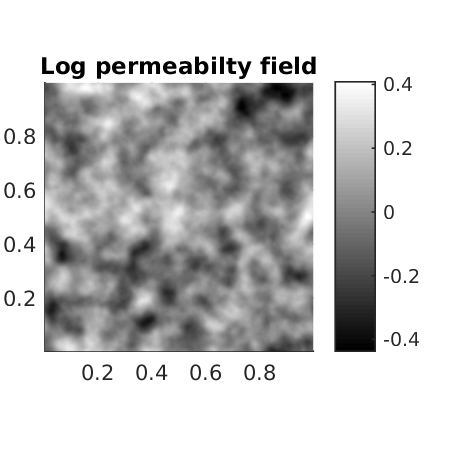
\includegraphics[scale=0.75]{figs/kfield_01_0025_0025.png} &
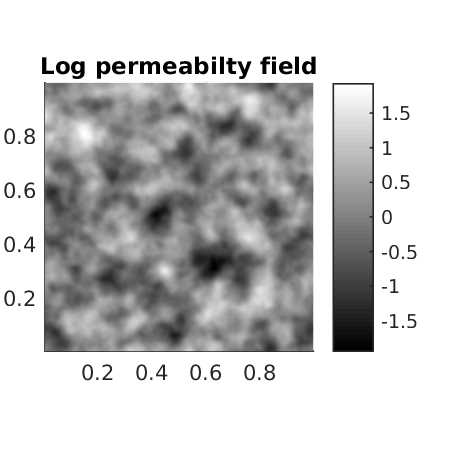
\includegraphics[scale=0.75]{figs/kfield_2_0025_0025.png} &
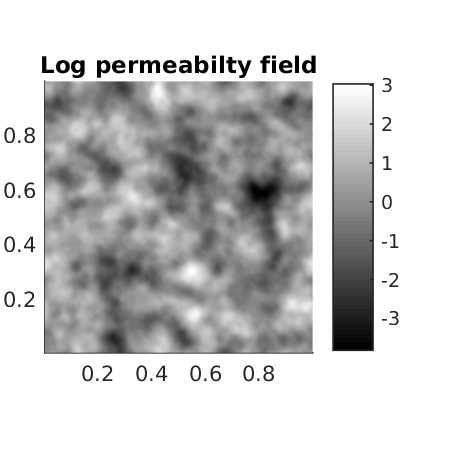
\includegraphics[scale=0.75]{figs/kfield_5_0025_0025.png}
\end{tabular}
\caption{Here the variance in log of k varies from 0.1 to 2 to 5 (left to right). The correlation lengths are both $5dx$, where $dx = 1/200$.}
\end{table}

Increasing the correlation length in these next images makes larger blocks of similar values.
\begin{table}[!h]
\centering
\begin{tabular}{c c c}
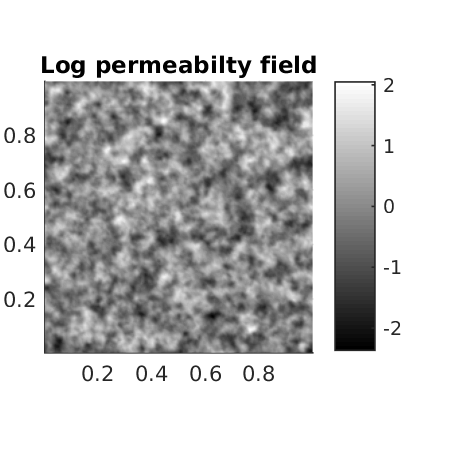
\includegraphics[scale=0.75]{figs/kfield_2_001_001.png} &
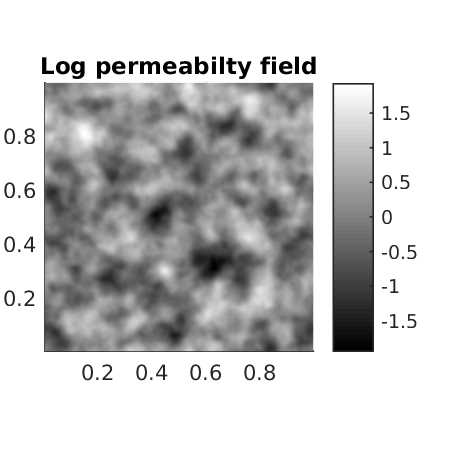
\includegraphics[scale=0.75]{figs/kfield_2_0025_0025.png} &
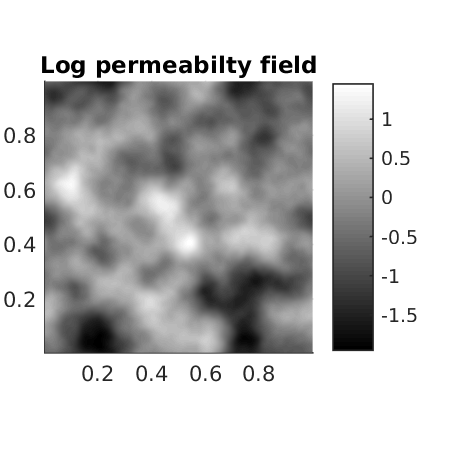
\includegraphics[scale=0.75]{figs/kfield_2_005_005.png}
\end{tabular}
\caption{Here the variance in log of k is constant at 2. The correlation lengths are equal to each other, but vary from $2dx$, to $5 dx$, to $20dx$ from left to right (again $dx = 1/200$).}
\end{table}


% \appendix
% \section{Programs}
% \lstinputlisting[label=code:plotting]{sandstone_figures.py}

\end{document}
